\documentclass[12pt]{article}
\usepackage[utf8]{inputenc}
\usepackage{amsmath}
\usepackage{times}
\usepackage{amsfonts}
\usepackage{amssymb}
\usepackage{graphicx}
\usepackage{tabularx}
\usepackage[font=small,labelfont=bf]{caption}
\usepackage[font=small]{subcaption}
\usepackage{wrapfig}
\usepackage[american]{babel}
\usepackage{csquotes}
\usepackage{xcolor}
\usepackage[style=apa,backend=biber,sorting=none]{biblatex}
\DeclareLanguageMapping{american}{american-apa}
\usepackage[section]{placeins}
\usepackage{rotating}
\usepackage{bbm}
\usepackage{latexsym}


\DeclareSourcemap{
  \maps[datatype=bibtex]{
    \map{
      \step[fieldset=abstract, null]
    }
  }
}

\addbibresource{fre.bib}
%\renewcommand\thesubsection{\alph{subsection}}


%\DeclareGraphicsExtensions{.eps,.png}

%%% margins 
\textheight 23.4cm
\textwidth 14.65cm
\oddsidemargin 0.375in
\evensidemargin 0.375in
\topmargin  -0.55in
%
\renewcommand{\baselinestretch}{2}
%
\interfootnotelinepenalty=10000
%
\renewcommand{\thesubsubsection}{\arabic{section}.\arabic{subsubsection}}
\newcommand{\myparagraph}[1]{\ \\{\em #1}.\ \ }
\newcommand{\parencitealtt}[1]{\parenciteauthor{#1},\parenciteyear{#1}}
\newcommand{\myycite}[1]{\parencitep{#1}}

% Different font in captions
\newcommand{\captionfonts}{\small \it}

\makeatletter  
\long\def\@makecaption#1#2{%
  \vskip\abovecaptionskip
  \sbox\@tempboxa{{\captionfonts #1: #2}}%
  \ifdim \wd\@tempboxa >\hsize
    {\captionfonts #1: #2\par}
  \else
    \hbox to\hsize{\hfil\box\@tempboxa\hfil}%
  \fi
  \vskip\belowcaptionskip}
\makeatother   
%%%%%

\begin{document}
\hspace{13.9cm}

\ \vspace{20mm}\\

{\LARGE Population activity encoding and transmission via traveling waves in neuronal systems}

\ \\
{\bf \large Vincent Baker, vjb42@drexel.edu$^{\displaystyle 1}$}\\
{\bf \large Luis Cruz, ccruz@drexel.edu$^{\displaystyle 1}$}\\
{$^{\displaystyle 1}$Drexel University, Department of Physics.}\\
%

%\ \\[-2mm]
{\bf Keywords:} Traveling waves,  minicolumns, population encoding

\thispagestyle{empty}
\markboth{}{NC instructions}
%
\ \vspace{-0mm}\\
%
%Abstract
\begin{center} {\bf Abstract} \end{center}
Information in the mammalian cortex is encoded in the firing activity of populations of neurons, and this information flows both within and between cortical regions.
Traveling waves of neuronal activity have also been shown to correlate with information transfer in the cortex.
Here we propose a mechanism for the encoding and transport of population activity via such traveling waves and demonstrate the mechanism in a simulation of cortical microcolumn structures.
We show that stimulus-evoked traveling waves in these microcolumn structures can encode the firing rate of a neuron population into the frequency of arrival of traveling waves.
We also investigate the resilience of such a mechanism to neuronal or synaptic damage and provide scaling approaches that make the structures resilient to damage while maintaining energy efficiency.

%%%%%%%%%%%

\section{Introduction} 
Individual neurons in the brain are tuned to fire upon specific events such as visual stimuli of a particular type \parencite{Hubel1962} .
However, even neurons that are tuned to a specific stimulus show variability in their firing rate and timing when the same stimulus is repeatedly applied \parencite{Georgopoulos1982}\parencite{Newsome1989}.
This indicates that information in the brain is represented by the firing dynamics of populations of many neurons.
This population coding may take the form of variations in the average firing rate of the neurons in the population (rate coding) or variations in the synchronization between spikes (temporal coding).
The temporal and rate coding ma also have a functional relation, i.e. through Hebbian learning \parencite{Basawaraj2019}.
Various methods of decoding the information in these population dynamics have been studied \parencite{Deneve1999}\parencite{Xu2019}, and population dynamics are incorporated into modern theories of neural computation \parencite{Pitkow2017}\parencite{Nadeau2020}.

Traveling waves of neuronal activation have been observed in the cortex as reviewed in \parencite{Muller2018}.
Various functional roles have been proposed for these traveling waves including spatiotemporal processing in the visual cortex \parencite{wu2008}\parencite{Muller2014}, place field coordination in the hippocampus \parencite{lubernov2009}, and memory consolidation during sleep \parencite{Dickey2021}.
Traveling waves have been shown to carry information in the  motor cortex \parencite{Rubino2006} and visual cortex \parencite{Besserve2015}.
These waves can provide synchronous activations of a population to serve functions such as gating perception of low-contrast images \parencite{Davis2020}.
In addition to extensive observations in vivo, traveling waves have also been observed in neuronal network simulations at the mesoscopic level in simple one-dimensional systems \parencite{Wilson1973}\parencite{Golomb1999} and two-dimensional sheets \parencite{keane2015}.
Traveling waves have also been studied in large-scale simulations of the entire brain \parencite{Roberts2019}.

Previous studies have used one-dimensional structures largely for their computational or analytic simplicity. 
Consideration of a quasi one-dimensional system may seem as an unnecessary complication, but there is no a priori reason that quasi one-dimensional traveling waves may not be found in vivo.
Of interest, there are regions of the brain where there are what seem to be quasi one-dimensional structures \parencite{mountcastle1997}\parencite{Cruz2009} typically called micro- or minicolumns. 
These minicolumns are aligned perpendicular to the pia and can be hundreds of microns long.  
Although their relevance to cognition and function is still being debated \parencite{horton2005}\parencite{buxhoeveden2002}, it is possible that they can sustain traveling waves.

Here we consider how quasi one-dimensional neuronal structures could encode and transmit population activity via traveling waves.
We perform computational experiments using a quasi one-dimensional model we cal a Small Columnar Ensemble (SCE), first reported in , with a network of Izhikevich neurons \parencite{izhikevich2003} using the same local connectivity model as \parencite{maass2002}.
We have previously shown that this model supports stimulus-evoked traveling waves across a variety of model parameters.
We now demonstrate that input from a population of neurons, simulated as Poisson spike trains, can evoke traveling waves in our quasi one-dimensional system.
The number of waves per second that span the SCE, which we term the wave arrival rate, increases as the average firing rate of the input pool of neurons is increased.
The plot of wave arrival rate versus input population firing rate resembles the activation functions of either a single neuron or a population of neurons.
This leads us to consider the SCE to have a nonlinear activation function in terms of input population rate, and to consider the SCE as encoding the input population firing rate into the wave arrival rate.

Just as a single neuron may be susceptible to noise or damage, a single SCE may also be an unreliable means of encoding and transmitting population rate information.
We therefore look at morphologies of multiple redundant SCE to enable reliable encoding and transport.
We find that simply increasing the cross-section of the SCE ...

\section{Methods}
To study traveling waves in small columnar ensembles (SCE) of neurons  we created a MATLAB simulation of our model based on \parencite{izhikevich2003}  . 
We first construct these assemblies by placing neurons at the vertices of a cubic lattice described by two short   dimensions (X,Y) and one long dimension (Z) . 
Each neuron is randomly chosen to be either excitatory (E) or inhibitory (I), with the fraction of excitatory neurons indicated as $P_{exc}$.
After placing, we connect two neurons based on their relative distance according to a connection probability that favors local connectivity described in \parencite{maass2002}: 
\begin{align}\label{eq:connectivity}
 P_{a,b} &= C e^{-(D(a,b)/\lambda)^2}
\end{align}
where $D(a,b)$ is the Euclidean distance between neuron A and B, $\lambda$ is the characteristic length of the local connectivity neighborhood, and $C$ is  the peak probability of connection  .
In \parencite{Levy2012} the authors showed that the synaptic connections in the mouse auditory cortex follow this connection probability.
Multiple connections from the same presynaptic neuron to the same postsynaptic neuron, as well as self-connections, are prohibited.
Two neurons may be recurrently connected, however. 
An example of an SCE showing the connectivity structure is shown in Figure \ref{fig:column_structure}.
\begin{figure}[!htb]
 \caption{Example SCE with dimensions 2x2x10 (X/Y/Z), $\lambda$=2.5, and C=1. A) SCE showing connections between neurons as lines colored using a color scale that indicates the connection length. 
 B) Connection matrix. E-E connections are green, E-I are black and both I-E and I-I are red. 
 The labels of the neurons used in both axes are sequentially assigned starting at the bottom (Z=0).}
 \label{fig:column_structure}
 \begin{subfigure}{0.3\textwidth}
   \centering
   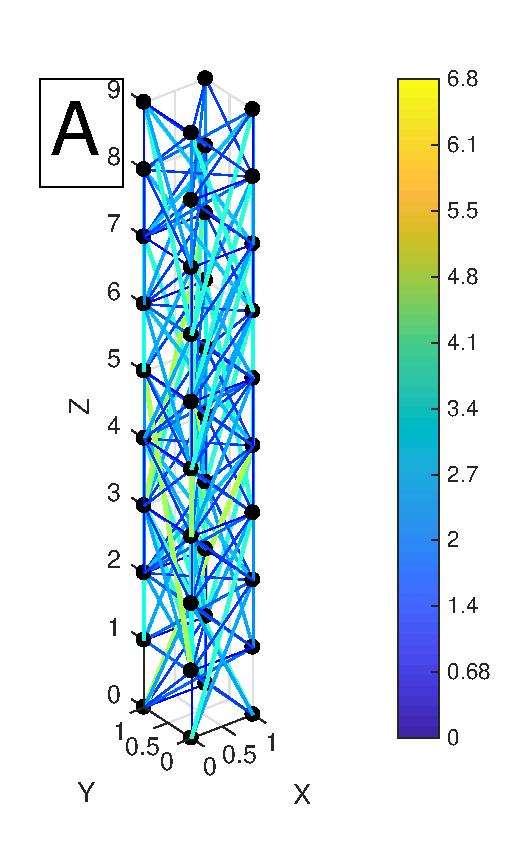
\includegraphics[height=60mm]{fig/column_structure_A}
 \end{subfigure}%
 \hfill
 \begin{subfigure}{0.7\textwidth}
   \centering
   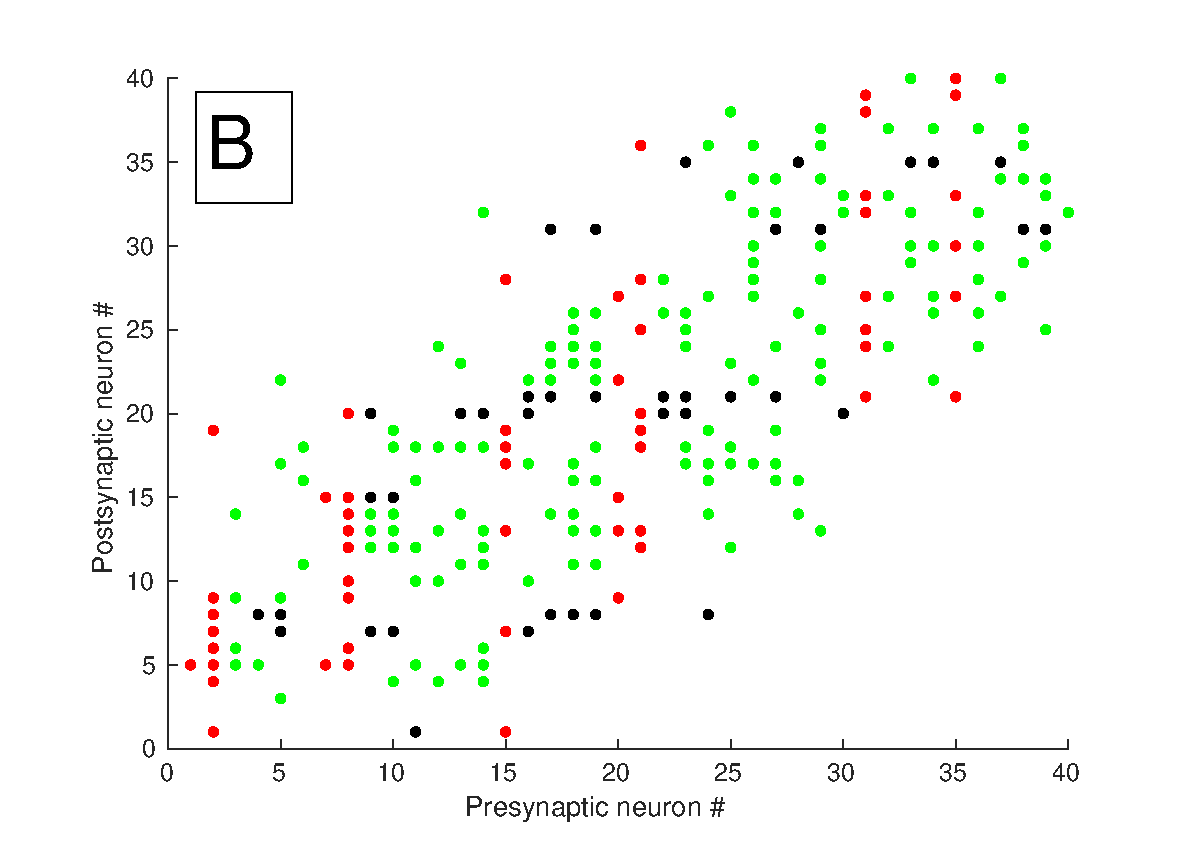
\includegraphics[height=60mm]{fig/column_structure_B}
 \end{subfigure}%
 \hfill
\end{figure}
We use open boundary conditions, so neurons near the ends of the SCE will have fewer connections than those in the middle. 

We model the firing dynamics of each neuron using the Izhikevich model \parencite{izhikevich2003} that consists of a two-dimensional model of two coupled differential equations given by:
\begin{align}
 \begin{split}
  v^\prime &= 0.04v^2+5v+140-u+I \label{eq:neuron_v} \\
  u^\prime &= a(bv-u)
 \end{split}
\end{align}
where $v$ is the membrane potential of the neuron and $u$ is a membrane recovery variable, with a spike threshold and an auxilliary after-spike resetting of parameters by:
\begin{align}
  \text{if } &v>30: v\leftarrow c, u\leftarrow u+d
\end{align}
and I is the sum of all incoming currents to the neuron, explained in detail below. 

Equation \ref{eq:neuron_v} has four parameters (a,b,c,d) that with specific values can model a wide range of neuronal spiking behavior \parencite{izhikevich2003}. 
The parameters used here (see Table \ref{tab:izzy_params}) are based on those specified in \parencite{izhikevich2003} with modification of the $c$ parameter for excitatory neurons and define a random population of neurons where $U(s,t)$ represent a number drawn from a uniform random distribution between s and t. 
\begin{table}[!htb]
 \caption{Izhikevich model parameters}
 \label{tab:izzy_params}
 \centering
 \begin{tabular}{l|c|r}
  \textbf{Parameter} & \textbf{Excitatory} & \textbf{Inhibitory} \\
  \hline
  a & 0.02 & 0.02+$\mathcal{U}$(0,0.08) \\
  b & 0.2 & 0.25-$\mathcal{U}(0,0.05)$\\
  c & -65+$\mathcal{U}(0,10)^2$ & -65 \\
  d & 8-$\mathcal{U}(0,6)$& 2 \\
 \end{tabular}
\end{table}
For solving equation (2) numerically we use the modified Euler method from \parencite{izhikevich2003} with a time step of $0.2 ms$ except were noted. 

A crucial element to evoke traveling waves in neuronal systems is the existence of time delays between the creation of a presynaptic action potential and the arrival of that spike to a target neuron. 
For this, we use distance-dependent time delays for the propagation of a spike from neuron $i$ to neuron $j$ of $\tau_{ij} = \kappa  D(i,j)$. 
 
The constant of proportionality $\kappa$ ranges from $0$ to $4$.
When $\kappa=0$ the action potential excites the post-synaptic neuron on the succeeding simulation time step.
 

The current I in equation (2) includes the sum of all incoming stimuli into neuron $i$ from other neurons $I_i$ and external stimuli $I_{i,e}$ applied to the system. 
The neuron-neuron incoming current $I_i$ into neuron $i$ is given by:
\begin{align}
 I_i(t) &= \sum_{j\ne i} \sum_{t^\prime_j} S_{ij}  \Theta(t-t^\prime_j-\tau_{ij})e^{-(\frac{t-t^\prime_j-\tau_{ij}}{\sigma_s})^2}
\end{align}

where $t'_j$ are the firing times of neuron $j$, $\Theta$ is the Heaviside step function, and the exponential factor models an exponentially decaying synapse response with a time constant of $\sigma_s = 4 ms$. 
The $S_{ij}$ represent the connection strengths between presynaptic neuron $j$ and postsynaptic neuron $i$ given by
\begin{align}
 \begin{split}
  S_{ij}^{excitatory} &= K \times \mathcal{U}\{0,0.5 \} \\
  S_{ij}^{inhibitory} &= K \times \mathcal{U}\{-1,0 \} 
 \end{split}
\end{align}

where $K$ is a parameter that modulates the strength of connections, with $K=1$ corresponding to the original model in \parencite{izhikevich2003}. 

\FloatBarrier

\section{Results}

\begin{figure}[!htb]
 \centering
 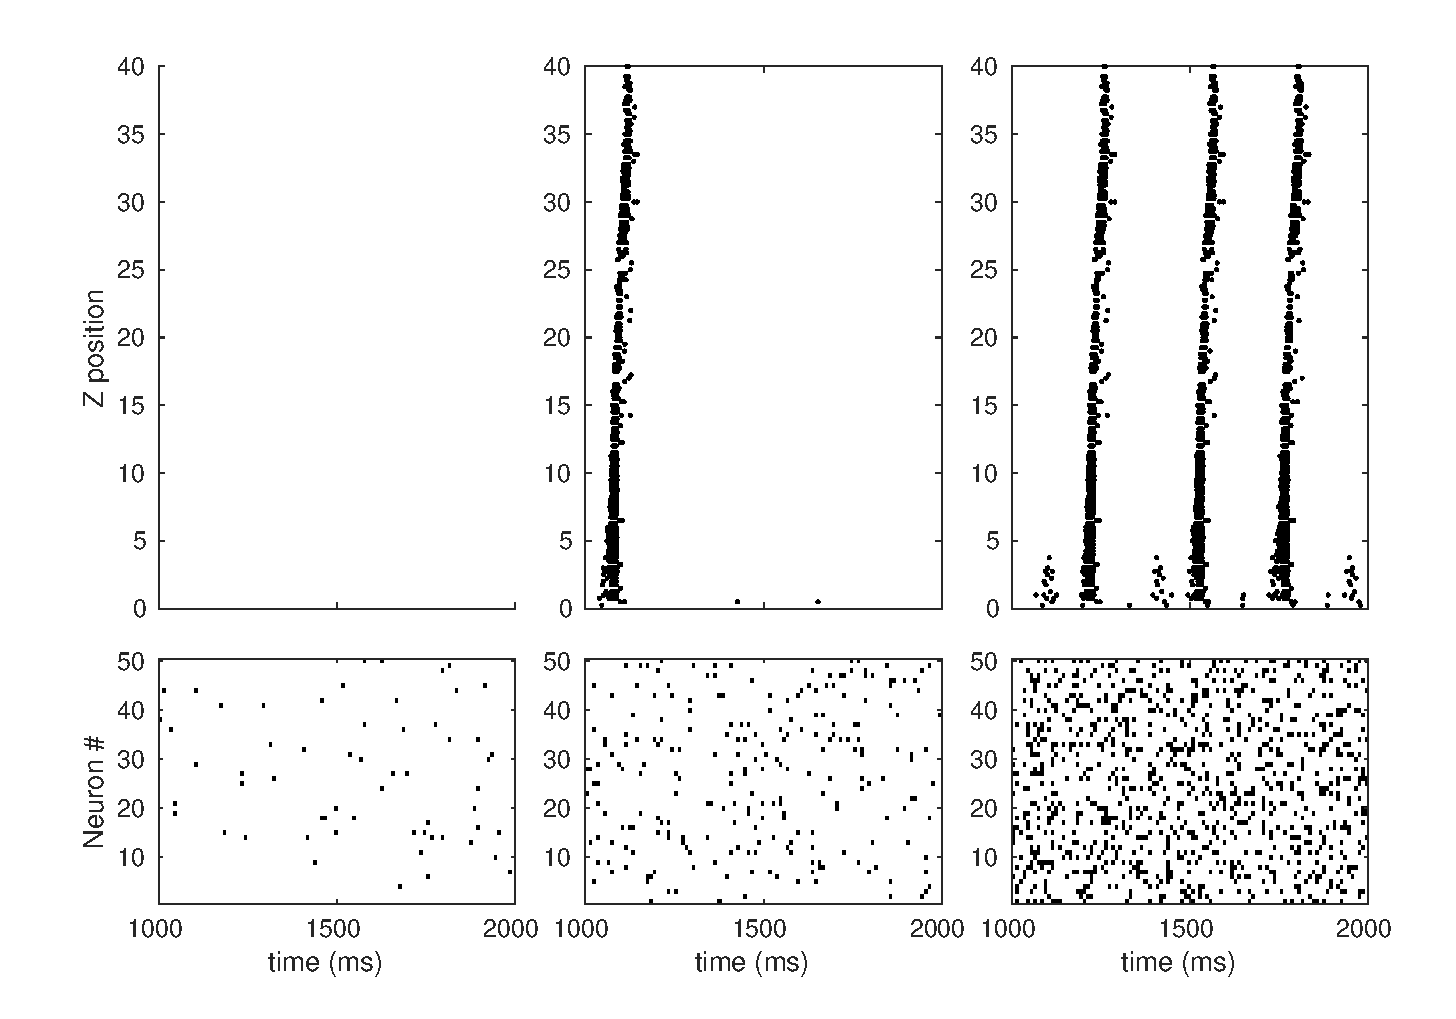
\includegraphics[width=\textwidth]{fig/SCE_2x2_FRE_rasters}
 \caption{Poisson spike trains in the input population (bottom) evoke traveling waves in the SCE (top). Raster plots are shown for firing rates of 1 spike/second (left), 5 spikes/second (middle) and 21 spikes/second (right).  }
 \label{fig:sce_raster}
\end{figure}

\begin{figure}[!htb]
 \centering
 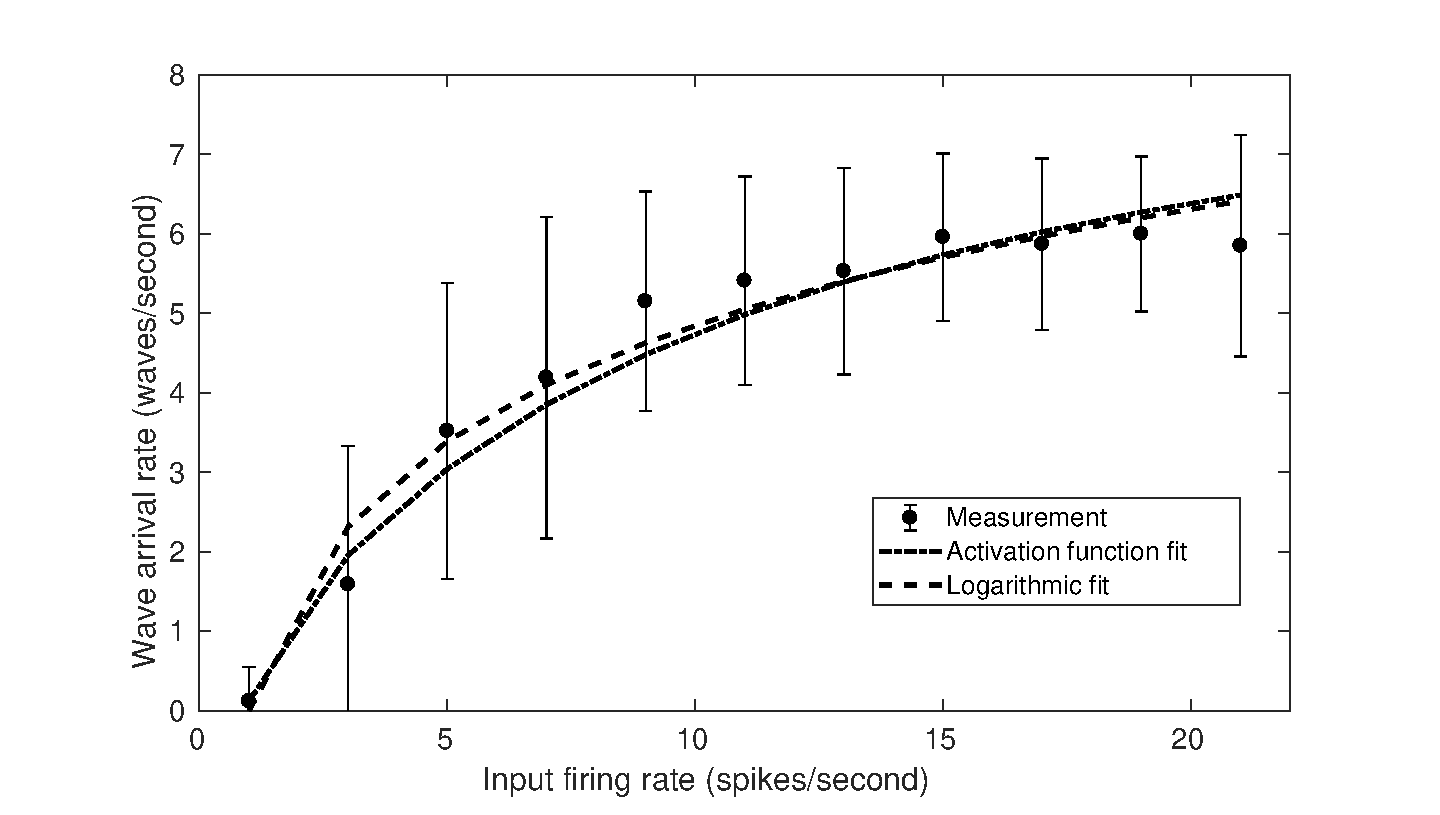
\includegraphics[width=\textwidth]{fig/SCE_2x2_FRE}
 \caption{The SCE encodes the input population firing rate into the wave arrival rate. }
 \label{fig:sce_activation_function}
\end{figure}

\section{Discussion}


\clearpage
\printbibliography

\end{document}
